\documentclass[oneside]{book}
\usepackage{hyperref}
\usepackage{subfiles}
\usepackage[utf8]{inputenc}
\usepackage{geometry}
\usepackage{graphicx}
\usepackage{titling}
\usepackage{datetime2}
\usepackage{fancyhdr}
\usepackage{lipsum}  
\usepackage{lmodern}
\usepackage{amssymb}
\usepackage{amsmath}
\usepackage{tikz}
\usepackage{listings}
\usepackage{float}
\usepackage{amsthm}

% 定义高亮命令
\newcommand{\grayhl}[1]{%
  \tikz[baseline=(text.base)]{%
    \node[rectangle, fill=gray!30, rounded corners, inner sep=2pt] (text) {#1};%
  }%
}

\usetikzlibrary{fadings, shadows}
 \geometry{
 a4paper,
 total={170mm,257mm},
 left=20mm,
 top=20mm, % 减小顶部边距,帮助标题置顶
 }
\author{Zewan LYU(999019888)}
\date{\today} % 恢复日期定义,但不在标题中显示
\title{Metric and Topological Space}
\fancypagestyle{plain}{%
    \fancyhf{} % 清除所有页眉页脚
    \fancyhead[L]{}
    \fancyhead[R]{\leftmark \ \ \ \grayhl{\ \ \ \thepage}}
}

\fancypagestyle{assignment}{%
    \fancyhf{} % 清除所有页眉页脚
    \fancyhead[L]{\theauthor}
    \fancyhead[R]{\leftmark \ \ \ \grayhl{\ \ \ \thepage}}
}

\renewcommand{\headrulewidth}{0.4pt}

\graphicspath{{images/}}

\hypersetup{
    colorlinks=true,
    linkcolor=blue,
    citecolor=green,
    urlcolor=cyan
}

\lstset{
  basicstyle=\ttfamily\small,
  keywordstyle=\color{blue},
  commentstyle=\color{green},
  numbers=left,
  frame=tb,
  breaklines=true
}

\newtheorem{theorem}{Theorem}[section]  % [section] 表示按章节编号(如 1.1)
\newtheorem{definition}{Definition}[section]
\newtheorem{example}{Example}[section]
\newtheorem{property}{Property}[section]
\newtheorem{corollary}{Corollary}[section]

% 保存原始环境的开始和结束命令
\let\oldtheorem\theorem
\let\endoldtheorem\endtheorem

% 重定义定理环境,自动添加标签
\renewenvironment{theorem}[1][]{%
  \oldtheorem[#1]% 开始原始定理环境,保留可选标题
  \label{thm:\thetheorem}% 自动创建标签:thm:编号(如thm:1.1.1)
}{%
  \endoldtheorem% 结束原始定理环境(正确语法)
}

\begin{document}

% -------------------------- 封面设计 --------------------------
\begin{titlepage}
    \centering % 所有内容居中对齐
    
    % 1. 顶部留白(根据页面比例微调,确保整体平衡)
    \vspace*{2cm}
    
    % 2. 核心 TikZ 曼陀罗图案(缩放至合适尺寸,避免过大/过小)
    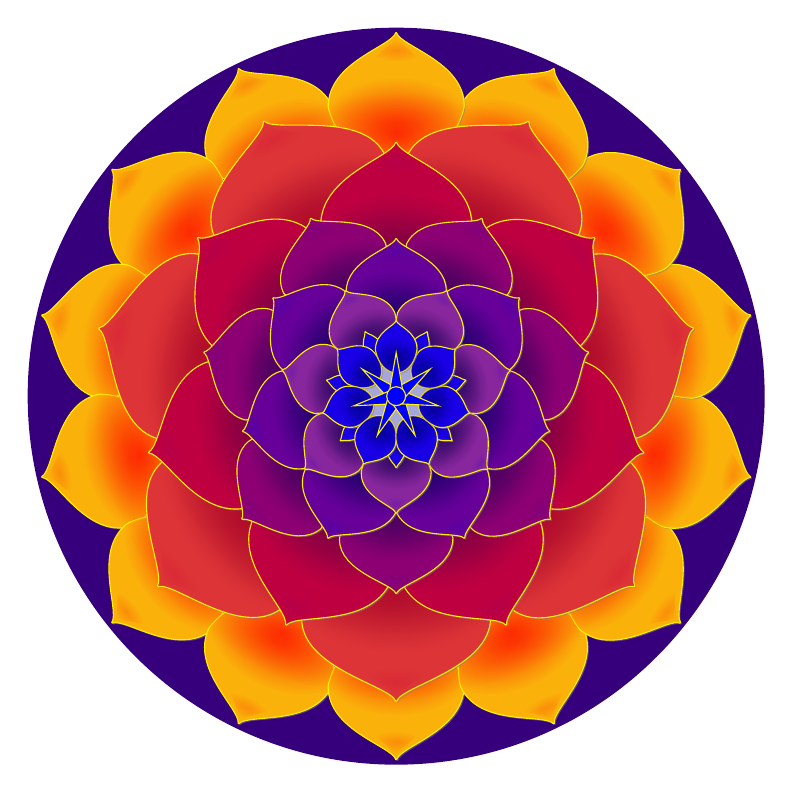
\begin{tikzpicture}[scale=1.2] % scale 控制图案整体大小
        % 曼陀罗图案定义(保留原代码逻辑,确保图案完整)
        \tikzfading[name=fade out, inner color=transparent!0, outer color=transparent!100]
        \def\petal { 
            [rounded corners=0.5]
            (-1,0).. controls (-1,0.6) and (-0.07,0.8).. (0,1)
            .. controls (0.07,0.8) and (1,0.6).. (1,0)
            .. controls (0.7,-1) and (-0.7,-1).. (-1,0)
        }
        \def\background[#1,#2]{
            \fill[#1] (0,0) circle (3.9);
            \fill[#2] (0,0) circle (1);
        }
        \def\center[#1]{
            \foreach \a in {51.4285,102.857,...,360} {
                \draw[color=yellow,rotate=\a,fill=#1] (-0.08,0) -- (0,0.46) -- (0.08,0);
            }
            \draw[color=yellow,fill=#1] (0,0) circle (0.1);
        }
        \def \mandala {
            \background[red!30!blue!70!black,blue!70!yellow!50];
            \foreach \ysh/\xs/\ys/\af/\as/\y/\b/\w/\r/\bl in {
                3.06/0.72/0.8/25.71425/51.4285/70/100/100/100/100,
                2.34/1/0.9/25.71425/77.14275/6/90/92/80/80,
                1.8/0.8/0.9/51.4285/102.857/0/75/100/60/70,
                1.5/0.6/0.6/25.71425/77.14275/0/55/100/40/60,
                1.1/0.53/0.58/51.4285/102.857/0/40/100/20/50,
                0.8/0.37/0.45/25.71425/77.14275/0/45/85/20/40,
                0.53/0.1/0.24/25.71425/77.14275/0/10/100/0/30,
                0.49/0.22/0.32/51.4285/102.857/0/10/100/0/50
            } {
                \foreach \a in {\af,\as,...,360} {
                    \begin{scope}[rotate=\a,shift={(0,\ysh)},xscale=\xs,yscale=\ys]
                        \draw[color=yellow,fill=yellow!\y!red!\b!blue!\w,
                              drop shadow={shadow xshift=0.5pt, shadow yshift=-0.5pt}]
                        \petal;
                    \end{scope}
                    \begin{scope}[transform canvas={rotate=\a},shift={(0,\ysh)},xscale=\xs,yscale=\ys]
                        \clip \petal;
                        \fill[path fading=fade out,fill=red!\r!blue!\bl!black, opacity=0.7]
                        (0,-0.35) ellipse (1.2 and 0.75);
                        \fill[path fading=fade out,fill=red!\r!blue!\bl!black, opacity=0.3]
                        (0,-0.2) ellipse (1.2 and 0.4);
                        \fill[path fading=fade out,fill=red!\r!blue,opacity=0.2]
                        (-0.4,0.6) -- (0,0.9) -- (0.4,0.6);
                    \end{scope}
                }
            }
            \center[blue]
        }
        % 绘制曼陀罗图案(核心视觉元素)
        \mandala;
    \end{tikzpicture}
    
    % 3. 文字信息区域(与图案保持适当间距,层次分明)
    \vspace*{1.5cm} % 图案与标题的间距
    
    % 主标题(加粗、大号字体,突出核心)
    {\Huge \bfseries \thetitle \par}
    
    % 副标题(比主标题小一号,灰色调,辅助说明)
    {\Large \color{gray!60} Mathematics With Computer Science \par}
    
    % 留白分隔(区分标题与作者信息)
    \vfill
    
    % 作者信息(中等字体,清晰易读)
    {\Large \textit{Author:} \theauthor \par}
    
    % 日期信息(使用 \today 自动获取当前日期,与作者对齐)
    {\Large \textit{Date:} \today \par}
    
    % 底部留白(确保封面底部不拥挤)
    \vspace*{1cm}
\end{titlepage}
% -------------------------- 封面结束 --------------------------

\pagestyle{plain}
\tableofcontents

\subfile{chapter1.tex}

\end{document}
